\section{Architektura systému}
\label{sec:kelvin-architecture}

Systém Kelvin je realizován jako webová aplikace se standardním třívrstvým uspořádáním: databázová vrstva, backendová aplikační logika a frontendová prezentační vrstva.
Komunikace mezi frontendem a backendem probíhá přes REST API (Representational State Transfer, Application Programming Interface)\@.

\subsection{Backend}
\label{subsec:kelvin-backend}

Backend systému je implementován v programovacím jazyce Python s využitím webového frameworku Django.
Django zajišťuje správu databázových modelů prostřednictvím ORM (Object-Relational Mapping), autentizaci a autorizaci uživatelů, správu souborů (odevzdaných zdrojových kódů a testovacích dat) a základní routování požadavků.

Použitým databázovým systémem je PostgreSQL, přičemž veškerý přístup k němu probíhá výhradně přes Django ORM\@.
Soubory zdrojových kódů jsou ukládány na souborový uložišti serveru, přičemž v databázi jsou uloženy pouze metadata (cesty, časové razítka, vazby na studenty a úlohy).

\subsubsection*{Evaluační pipeline}
\label{subsubsec:kelvin-evaluation-pipeline}

Stávající evaluační pipeline systému zajišťuje kompilaci odevzdaného zdrojového kódu a spuštění automatických testů v izolovaném prostředí.
Izolace je realizována prostřednictvím kontejnerů (Docker) a omezení přístupu k systémovým zdrojům, což chrání infrastrukturu před škodlivým nebo nekorektním kódem a současně garantuje jednotné podmínky evaluace pro všechny studenty.
Vyhodnocení je implementováno jako asynchronní úloha z pohledu aplikační architektury, nicméně z hlediska uživatelského chování se jedná o proces synchronní, protože student čeká na jeho dokončení před zobrazením výsledků testů.

Zařazení dalších výpočetně náročných operací přímo do této pipeline, například generování analýzy pomocí velkých jazykových modelů, by vedlo k prodloužení doby čekání na výsledek.
I pokud by byly tyto operace realizovány technicky asynchronně, jejich začlenění do stejného evaluačního procesu by mělo přímý dopad na vnímanou latenci systému uživatelem.

Vedle evaluační pipeline systém Kelvin provádí rovněž kontrolu plagiátorství.
Ta je ze své podstaty vázána na celou skupinu odevzdání, nikoli na jedno konkrétní, a je proto spouštěna buď manuálně učitelem, nebo automaticky po vypršení termínu odevzdání dané úlohy.
Po spuštění systém porovná každé odevzdání s každým ostatním ve skupině za využití nástrojů DOLOS a MOSS\@.
Díky tomuto uspořádání kontrola plagiátorství nijak neovlivňuje dobu čekání studentů na výsledky automatických testů.

\subsection{API vrstva}
\label{subsec:kelvin-api}

Komunikace mezi frontendem a backendem probíhá prostřednictvím REST API implementovaného za pomocí knihovny Django Ninja.
Django Ninja je moderní framework pro budování API nad Django, inspirovaný FastAPI, který využívá Python \textit{type hints} pro automatickou validaci vstupních dat a generování OpenAPI dokumentace přístupnou například přes Swagger UI\@.

\subsection{Frontend}
\label{subsec:kelvin-frontend}

Frontendová část systému je z technologického hlediska výrazně komplikovanější než backend, protože prochází historickým vývojem, který zanechal vrstvení tří různých technologií v jednom projektu.

Nejstarší vrstvou jsou \textit{Django šablony} (Django templates) -- serverově generované HTML stránky, které byly původním způsobem tvorby uživatelského rozhraní.
Django šablony jsou stále přítomny v systému u statičtějších částí rozhraní, kde není potřeba dynamického chování na straně klienta.

Druhou vrstvou je \textit{Svelte} -- moderní JavaScript framework pro tvorbu reaktivních komponent na straně klienta.
V průběhu vývoje systému Kelvin byl Svelte adoptován jako primární framework pro dynamické části rozhraní, zejména pro zobrazení a přidávání komentářů ke zdrojovému kódu.
Svelte komponenty jsou v produkci kompilovány do čistého JavaScriptu bez runtime knihovny, což zajišťuje rychlé načítání.

Třetí a v současnosti preferovanou vrstvou je \textit{Vue.js} -- progresivní JavaScript framework, na který systém v současné době systém migruje.
Vue.js bylo zvoleno jako nástupce Svelte zejména z důvodu větší komunity, lepší dlouhodobé podpory a nižší vstupní bariéry pro nové přispívatele.

Výsledkem tohoto historického vývoje je stav, kdy se ve zdrojovém kódu systému souběžně nacházejí všechny tři frontendové technologie.
Dopady tohoto stavu na vývoj nových funkcionalit jsou rozvedeny v \secref[sekci]{sec:kelvin-development}.

\begin{figure}[ht]
    \centering
    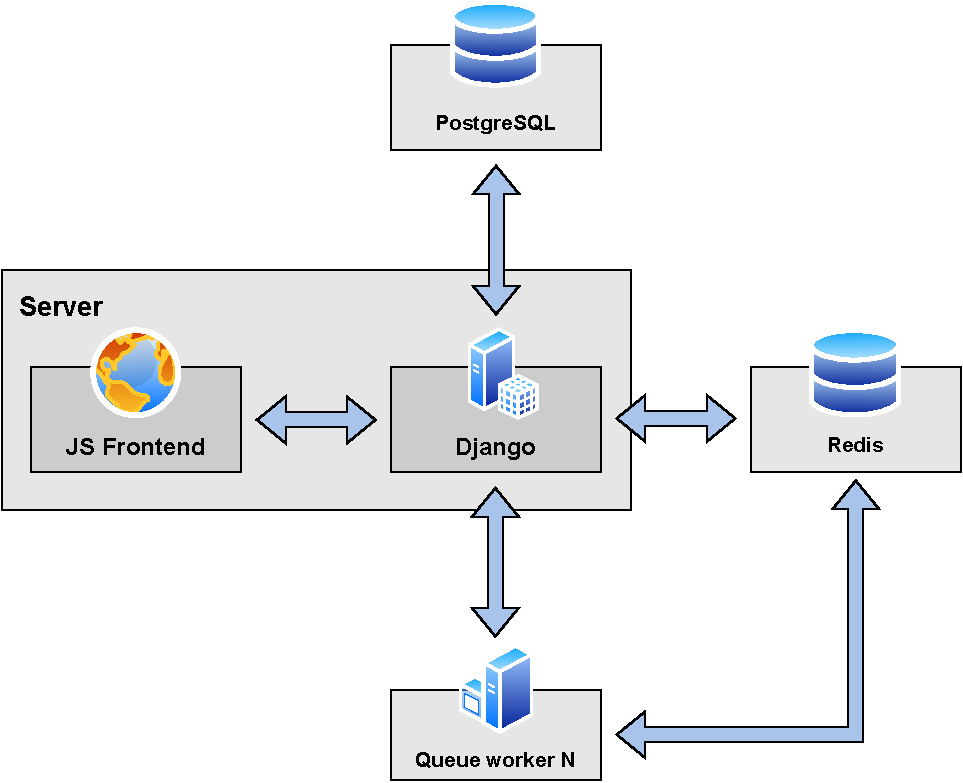
\includegraphics[width=0.85\textwidth]{resources/diagrams/kelvin-architecture}
    \caption{Zjednodušená architektura systému Kelvin~\cite{kelvin-architecture}}\label{fig:kelvin-architecture}
\end{figure}

\endinput